\section{Metodologia}
\label{sec-metodo}
Este estudo tem como objetivo aprimorar a busca por soluções para o problema da Árvore Geradora com Número Mínimo de Vértices d-branch (d-MBV). Para isso, a metodologia proposta integra a meta-heurística ILS (\textit{Iterated Local Search}), aprimorada em \cite{silva2024ils}, com a abordagem apresentada em \cite{lima2024ils}. Além disso, o trabalho também explora outras meta-heurísticas consolidadas na literatura, como \textit{Multi-Start} e GRASP, descritas brevemente na seção anterior, a fim de comparar seu desempenho na busca de soluções para o problema.

\subsection{O Problema d-MBV}
\label{dMBV}

A formulação do problema MBV inicia-se com um grafo \( G \) conexo, não direcionado e não ponderado, caracterizado por seu conjunto de vértices \( V_G \) e arestas \( E_G \). O objetivo central é identificar uma árvore geradora \( T = (V_T, E_T) \), na qual \( V_T = V_G \) e \( E_T \subseteq E_G \), que minimize o total de vértices com grau superior a \( 2 \) dentro dessa árvore. Tais vértices são designados como vértices \textit{branch} ou pontos de ramificação. A introdução do problema MBV por \citep{gargano:2002} foi motivada pela necessidade prática de otimizar a alocação de \textit{switches}. A minimização do número de vértices \textit{branch} é de crucial importância, visto que o custo associado a esses dispositivos é substancial, e a redução de sua quantidade pode gerar economias significativas.

Posteriormente, em \cite{merabet:2018}, o conceito de \textit{k-branch} foi proposto, representando uma generalização do problema MBV. Nessa definição, um vértice é classificado como \textit{k-branch} se seu grau excede estritamente \( k + 2 \). Assim, o problema k-MBV objetiva encontrar a árvore geradora que minimize o número de vértices \textit{k-branch}. Os autores dessa generalização demonstraram que o problema permanece NP-Difícil para qualquer valor de \( k \). Visando simplificar a notação, \cite{morenotese:2018} introduziu o parâmetro \( d = k + 2 \). Com essa nova designação, um vértice em um grafo é classificado como \textit{d-branch} se seu grau for estritamente maior que \( d \), para $d \ge 2$. Consequentemente, o problema d-MBV herda os objetivos e conceitos do problema MBV original, focando na minimização do número de vértices \textit{branch} nas soluções.




\subsection{Estudo sobre a Relação de Densidade e Vértices \textit{branch} em um Grafo}
\label{sec-metodo-densidade}

A partir de uma intuição inicial, é notável a existência de uma relação inversa entre a densidade de um grafo e a quantidade de vértices \textit{branch}. Em grafos densos, a alta conectividade distribui melhor as arestas entre os vértices, reduzindo a probabilidade de concentração em poucos pontos e, consequentemente, a formação de vértices \textit{branch}. No limite, os grafos completos, que apresentam densidade máxima e distribuição totalmente homogênea de conexões, evidenciam esse comportamento. Formalmente, a densidade de um grafo não orientado $G$ é definida pela razão entre o número de arestas $m$ e o número máximo possível de arestas em um grafo com $n$ vértices, sendo expressa por $\text{densidade}(G) = \frac{2m}{n(n - 1)}$.

Com base nessa definição, \cite{lima2024ils} investigou a relação entre densidade e número de vértices \textit{branch}, utilizando instâncias com soluções exatas conhecidas. A análise empírica revelou um comportamento semelhante a uma função de proporção inversa, como $f(x) = 1/x$. Essa evidência sugere uma dependência não linear e inversamente proporcional entre o número de vértices \textit{branch} e a densidade, conduzindo à seguinte modelagem aproximada:
\begin{equation}
db(G) \approx \frac{1}{K \times \text{densidade}(G)}
\label{eq:densidadeXalfa}
\end{equation}
em que $db(G)$ representa a quantidade de vértices \textit{branch} em $G$, e $K$ é um parâmetro de ajuste.  

\subsubsection{Determinação do Parâmetro $K$}
Na etapa seguinte, visando o aprimoramento do modelo proposto em \cite{lima2024ils}, dureante este trabalho realizou-se o ajuste do parâmetro $K$. Para isso, foi considerado o mesmo conjunto de instâncias com soluções exatas conhecidas, calculando $K$ para cada instância com a quantidade exata de vértices \textit{branch}, conforme estabelecido na Equação \ref{eq:calculo_k}:

\begin{equation}
\label{eq:calculo_k}
K = \frac{1}{db(G) \times \text{densidade}(G)}.
\end{equation}

A análise da distribuição dos valores obtidos indicou que $K$ não se comporta como uma constante, mas varia de acordo com propriedades estruturais do grafo. Diante dessa variabilidade, foi adotado uma abordagem de regressão linear \citep{seber2003linear} para estimar $K$. Essa abordagem possibilita capturar a relação entre o parâmetro e características relevantes do grafo, como número de vértices, arestas e densidade, fornecendo estimativas mais robustas e adequadas ao problema.


\subsection{Novo Algoritmo Construtivo}

Com base no estudo sobre a influência da densidade dos grafos no comportamento dos vértices \textit{branch} e na determinação do parâmetro $K$, foi possível propor uma nova abordagem que integra essas informações a contribuições anteriores da literatura. Em \cite{oliveira:2023}, foi implementado um algoritmo construtivo fundamentado em uma heurística randomizada, que apresentou bons resultados. Posteriormente, em \cite{silva2024ils}, a mesma heurística foi aprimorada com a inserção da centralidade \textit{PageRank}, demonstrando eficácia na identificação de vértices com maior probabilidade de se tornarem \textit{branch}.

A partir dessas duas direções de pesquisa, este trabalho propõe uma estratégia híbrida: combinar a estimativa da quantidade de vértices \textit{branch}, obtida por meio do densidade do grafo, com a seleção dos vértices mais promissores segundo a centralidade \textit{PageRank}. Para incorporar esses elementos, o algoritmo construtivo R-BEP (\textit{Randomized Branch Expanding Prim}) foi selecionado como base e modificado, de modo a explorar as características e informações estudadas durante este trabalho.

\subsubsection{Algoritmo Construtivo R-BEP}
\label{sec:rbep}
O R-BEP é um método para construir uma árvore geradora em um grafo $G$, composto por três fases principais:
\begin{itemize}
    \item \textbf{Identificação:} O algoritmo encontra e adiciona à solução parcial $T$ vértices que, se removidos, criariam três ou mais componentes conexas, tornando-os obrigatoriamente \textit{branch}.
    \item \textbf{Expansão:} Em seguida, os vértices já em $T$ são expandidos, incluindo todos os seus vizinhos e arestas. Essa expansão é possível pois o problema \textit{d}-MBV não impõe restrições ao grau máximo dos vértices.
    \item \textbf{Construção da Árvore Geradora:} Para completar a árvore com $|V|-1$ arestas, o R-BEP seleciona e expande iterativamente as "folhas" da árvore parcial, com pesos proporcionais aos seus graus no grafo original. Um novo vizinho é sorteado a cada passo até a árvore estar completa. Detalhes adicionais podem ser encontrados em \cite{oliveira:2023}.
\end{itemize}





\subsubsection{Algoritmo Construtivo R-PREV}
\label{sec:rprev}
A variação proposta modifica a fase inicial do algoritmo R-BEP, substituindo a seleção determinística de vértices obrigatórios por um processo baseado em estimativa e centralidade. O procedimento está descrito no pseudocódigo \ref{alg:rprev} e o funcionamento do algoritmo pode ser resumido em três etapas principais:


\begin{algorithm}

\caption{R-PREV}
\label{alg:rprev}
\SetAlgoLined
\Entrada{Grafo $G = (V, E)$, $\alpha = (0, 1)$.}
\Saida{Árvore Geradora $T = (V, E)$.}
$dbPREV \gets \text{Cálculo-dbPREV}(G)$;
\label{lin:calculo_dbPREV}\\
$(T, B_{\text{T}}, Pontas) \gets \text{Pré-Processamento}(G, dbPREV, \alpha)$;\label{lin:PreProcessamento}\\
\Enqto {$|E_{\text{T}}| < |V_{\text{G}}| - 1$}{ \label{lin:inicioloopRPREV}
    Sorteia um vértice $u \in \text{Pontas}$ com probabilidade proporcional ao seu grau $d(u)$ em $G$;\\
    Sorteia um vizinho $v \in N(u)$ que não forma ciclo em $T$;\\
    Adiciona a aresta $(u, v)$ a $T$;\\
    Atualiza Pontas e $B_{\text{T}}$;
}\label{lin:fimloopRPREV}
\textbf{return} $R$\;
\end{algorithm}



\begin{itemize}
    \item \textbf{Linha \ref{lin:calculo_dbPREV}:} 
    É executada a função \textit{Cálculo-dbPREV}, que utiliza as propriedades do grafo (número de vértices, arestas e densidade) para estimar a quantidade de vértices \textit{branch}. Essa estimativa, denotada por $dbPREV$, é obtida a partir da equação \ref{eq:densidadeXalfa} em conjunto com o parâmetro $K$ ajustada anteriormente.

    \item \textbf{Linha \ref{lin:PreProcessamento}:} 
    A função \textit{Pré-Processamento} recebe como entrada $G$, $dbPREV$ e $\alpha$. Inicialmente, todos os vértices do grafo $G$ são ordenados em ordem decrescente de acordo com sua centralidade \textit{PageRank}, formando o conjunto $S$. O parâmetro $\alpha$ define a fração de vértices de $S$ que estarão disponíveis para o sorteio: quando $\alpha = 1$, todo o conjunto é considerado, resultando em uma seleção altamente aleatória; quando $\alpha = 0$, apenas o vértice mais bem posicionado é escolhido, tornando o processo totalmente guloso. Assim, $\alpha$ atua como um regulador entre exploração (aleatoriedade) e intensificação (escolha determinística), permitindo a adoção de diferentes estratégias de construção. Em seguida, um subconjunto de tamanho $dbPREV$ é sorteado dentro de $S$ e inserido em $T$, compondo a solução parcial inicial. Esses vértices são diretamente classificados como \textit{branch} e adicionados ao conjunto $B_T$. A partir deles, inicia-se um processo de expansão que gera uma floresta parcial, cujas folhas formam o conjunto $Pontas$, ou seja, os vértices disponíveis para novas conexões sem aumento imediato no número de \textit{branch}.

    \item \textbf{Linhas \ref{lin:inicioloopRPREV} a \ref{lin:fimloopRPREV}:} A partir da solução parcial, a árvore é completada iterativamente. Em cada iteração, um vértice $u \in Pontas$ é escolhido com probabilidade proporcional ao seu grau e conectado a um vizinho $v$ que não forme ciclos. Essa seleção por sorteio prossegue até que $T$ contenha exatamente $|V|-1$ arestas. O processo segue a lógica original doR-BEP \citep{oliveira:2023}, garantindo conectividade e minimização do número de vértices \textit{branch}, que só são introduzidos quando estritamente necessário.

\end{itemize}

\subsection{Estratégias de Combinação de Algoritmos}
\label{sec-metodo-combinacao-algoritmos}

O pseudocódigo \ref{alg:frameworkMBV} serve como \textit{framework} para as estratégias híbridas exploradas neste estudo. Ele integra as ferramentas desenvolvidas, recebendo como entradas o grafo \textbf{$G$}, o parâmetro \textbf{$\alpha$} e o número máximo de iterações \textbf{$MaxIter$}. O grafo \textbf{$G$} representa a estrutura do problema, na qual se busca construir uma árvore $T$ que conecte todos os vértices com um subconjunto de arestas. O parâmetro \textbf{$\alpha$}, detalhado na Seção \ref{sec:rprev}, regula o espaço de vértices elegíveis para sorteios, balanceando entre a aleatoriedade e decisões gulosas. \textbf{$MaxIter$}, por sua vez, define o número de repetições do laço externo, influenciando a exploração e a intensificação do processo de busca.

O procedimento inicia com a inicialização de \textbf{$T^*$} (linha \ref{lin:InicializacaoT*}), responsável por armazenar a melhor solução global, seguida da geração de uma solução viável pelo algoritmo construtivo R-PREV (linha \ref{lin:SolucaoInicialHibrido}). Em seguida, essa solução é refinada por uma etapa de busca local (linha \ref{lin:BuscaLocal1Hibrido}), resultando em \textbf{$T_{local}$}. Entre as linhas \ref{lin:InicioLoopHibrido} e \ref{lin:FimLoopHibrido}, ocorre um ciclo iterativo de perturbação e busca local. A perturbação (linha \ref{lin:PertubacaoHibrido}) modifica a solução para escapar de ótimos locais, enquanto a busca local (linha \ref{lin:BuscaLocal2Hibrido}) explora a vizinhança em busca de melhorias. O critério de aceitação (linha \ref{lin:CriterioAceitacaoHibrido}) gerencia a transição entre soluções. O processo se repete até que a condição de parada seja satisfeita, que, neste trabalho, é a ausência de modificações válidas pela função de perturbação. Finalmente, a linha \ref{lin:VerificacaoHibrido} compara a solução obtida com a melhor solução conhecida. Se for superior, a nova solução é armazenada (linha \ref{lin:SalvandoSolucaoHibrido}), e o algoritmo prossegue para a próxima iteração.


\begin{algorithm}
\caption{Híbrido MBV}
\label{alg:frameworkMBV}
\SetAlgoLined
\Entrada{O grafo $G = (V, E)$, $\alpha = (0, 1)$, $MaxIter$.} \label{lin:EntradaILS}
\Saida{Uma solução válida $T$.}
$T^* \gets \emptyset$\;\label{lin:InicializacaoT*}
\Para{$i = 1$ \textbf{até} $MaxIter$}{ 
    $T_0 \gets RPREV(G, \alpha)$; \label{lin:SolucaoInicialHibrido} \\ 
    $T_{local} \gets Busca\_Local(T_0)$; \label{lin:BuscaLocal1Hibrido}\\
    \Repita{$condicao\ de\ parada\ atendida$}{\label{lin:InicioLoopHibrido}
        $T' \gets Perturbacao(T_{local})$; \label{lin:PertubacaoHibrido}\\
        $T'' \gets Busca\_Local(T')$; \label{lin:BuscaLocal2Hibrido}\\
        $T_{local} \gets Criterio\_Aceitacao(T_{local}, T'', historia)$; \label{lin:CriterioAceitacaoHibrido}\\   
    }\label{lin:FimLoopHibrido}
    \Se{$T_{local}$ é melhor que $T^*$}{ \label{lin:VerificacaoHibrido}
        $T^* \gets T_{local}$; \label{lin:SalvandoSolucaoHibrido}\\
    }
}
\textbf{return} $T^*$\;
\end{algorithm}

Inspirado no algoritmo \ref{alg:frameworkMBV} e em suas variações, a Figura \ref{fig:fluxograma} apresenta uma visão esquemática das estratégias combinadas desenvolvidas e implementadas neste estudo. As variações são detalhadas nas subseções seguintes.

\begin{figure}[h!]
    \centering
    \caption{\small Fluxograma das combinações de algoritmos aprimoradas e implementadas neste estudo pelo autor.}
    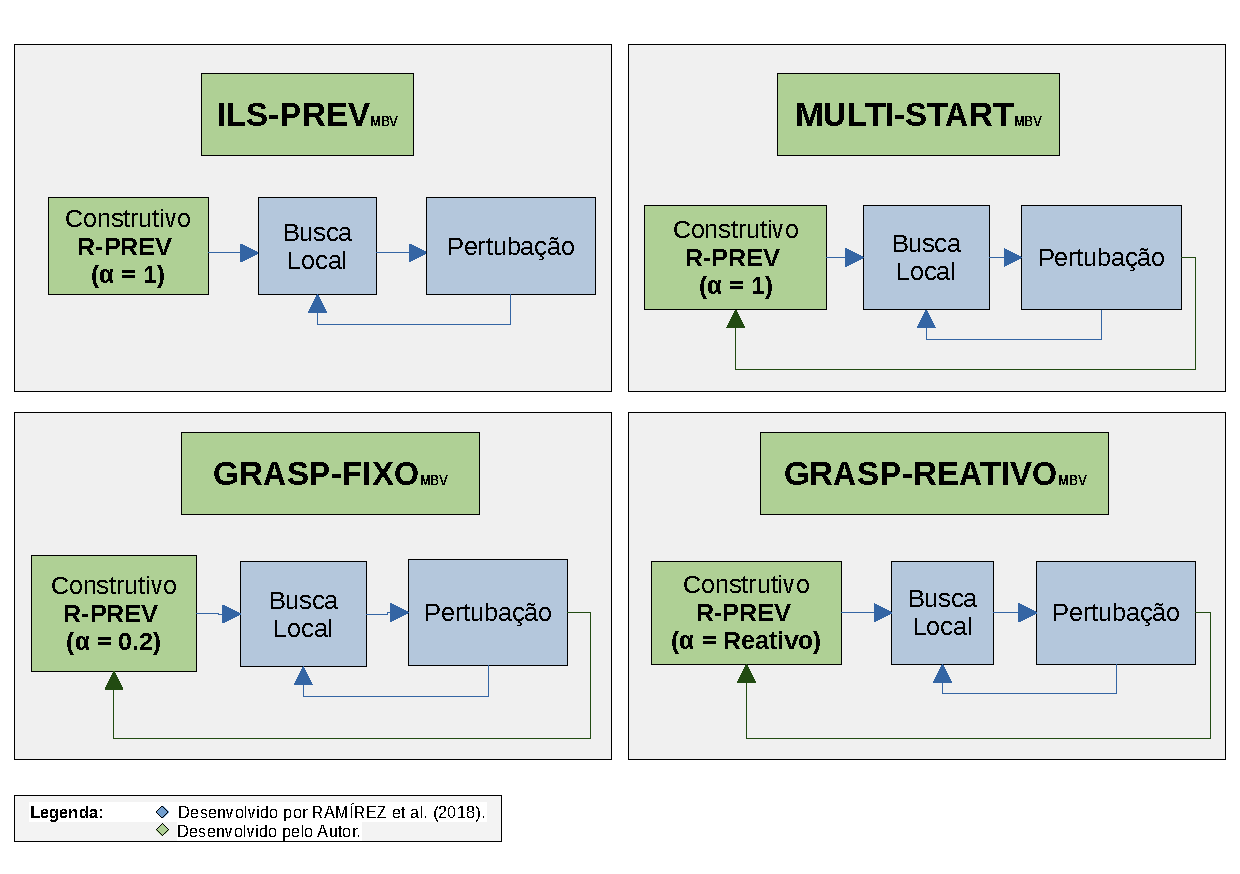
\includegraphics[width=13cm]{figuras/fluxograma.pdf}
    \caption*{\small Fonte: Produção do próprio autor.}
    \label{fig:fluxograma}
\end{figure}


\subsubsection{ILS-PREV {\small (MBV)}}

O ILS-PREV é uma especialização do Algoritmo \ref{alg:frameworkMBV} onde \textbf{$MaxIter = 1$}. A execução se restringe a um único ciclo do laço externo, o que o caracteriza como uma versão simplificada da meta-heurística ILS. A principal diferença em relação a trabalhos anteriores,  \cite{silva2024ils} e \cite{oliveira:2023}, reside no uso exclusivo do algoritmo R-PREV como método construtivo. Além disso, a configuração fixa $\alpha = 1$ promove um comportamento altamente aleatório, maximizando a diversidade na geração da solução inicial.


\subsubsection{MULTI-START {\small (MBV)}}

A estratégia Multi-Start explora o espaço de busca executando repetidamente um algoritmo construtivo simples a partir de diferentes pontos iniciais. No contexto deste trabalho, a variante do algoritmo R-PREV é utilizada múltiplas vezes. A melhor solução entre todas as execuções é selecionada como o resultado final. Esta estratégia é definida por \textbf{$MaxIter > 1$}, e por um valor fixo de $\alpha = 1$, o que confere ao processo de construção um caráter predominantemente aleatório. A variável \textbf{$MaxIter$} deve ser ajustada para encontrar o equilíbrio ideal entre tempo computacional e a qualidade da solução.



\subsubsection{GRASP-FIXO {\small (MBV)}}

O GRASP-FIXO é uma variante do \textit{Multi-Start} que compartilha a mesma estrutura de laço externo (\textbf{$MaxIter > 1$}) e algoritmo construtivo aleatório. Sua distinção fundamental é a utilização de um valor fixo de \textbf{$\alpha = 0,2$}. Esta variável restringe o sorteio de elementos para o algoritmo construtivo aos $20\%$ melhores vértices disponíveis, tornando-o mais restritivo que o \textit{Multi-Start}. A dependência de um $\alpha$ fixo pode impactar o desempenho, especialmente em instâncias de problemas que se beneficiariam de uma maior diversidade na busca.


\subsubsection{GRASP-REATIVO {\small (MBV)}}

O GRASP-REATIVO também é uma variante do \textit{Multi-Start} com a mesma estrutura básica, mas com uma inovação no tratamento de \textbf{$\alpha$}. Em vez de um valor fixo, o algoritmo aprende e se adapta durante a execução para encontrar o $\alpha$ ideal para cada tipo de instância, conforme proposto em~\cite{feo1995grasp}. O processo se dá em duas etapas:
\begin{enumerate}
    \item \textbf{Teste e Atribuição de Pesos:} Inicialmente, o algoritmo testa um conjunto de valores para $\alpha$ e avalia a qualidade das soluções geradas. Pesos são atribuídos a cada $\alpha$, com valores melhores recebendo pesos maiores.
    \item \textbf{Seleção Ponderada:} Nas iterações subsequentes, o $\alpha$ é sorteado por meio de uma roleta ponderada. Isso garante que os valores com maior peso (ou seja, aqueles que produziram as melhores soluções) tenham uma probabilidade maior de serem utilizados.
\end{enumerate}
Essa abordagem de aprendizado contínuo refina as escolhas ao longo do tempo. Consequentemente, quanto maior o número de iterações, maior a tendência de o GRASP-REATIVO encontrar soluções de alta qualidade.